\documentclass[10pt]{examdesign}
\usepackage{amsmath}
\usepackage{enumitem}
\usepackage{amsfonts}
\usepackage{pgfplots}
\usepackage{pifont}
\usepackage{graphicx}
\usepackage{fancyhdr}
\usepackage{cancel}
\usepackage[american]{circuitikz}

\SectionFont{\large\sffamily}
\Fullpages
\ContinuousNumbering
\usepackage{ulem}
\ProportionalBlanks{2}


\DefineAnswerWrapper{}{}
\NumberOfVersions{1}
%\IncludeFromFile{foobar.tex}
\examname{\Large{Horizontal Launch Projectiles}}
\class {\Large Physics}

\def \namedata {Name: \hrulefill\\ 
	Date: \hrulefill \\
	Period: \hrulefill \\
	Primary Peer Reviewer: \hrulefill 
	\\
			\begin{tabular}{| p{1cm} | p{1cm} | p{1 cm} | p{1cm} |}
	\hline
		+1 & 0 & -1 & $\Sigma$ 
		\\
		\hline
		& & & \vspace{.5cm}
		\\ \hline
	
	\end{tabular}
	\\
 \vspace{-.6in}
	
}




\begin{document}




\begin{multiplechoice} [title={Multiple Choice},
	rearrange=no]
	
\begin{block}
	The following information is for questions 1-2:
	
	
		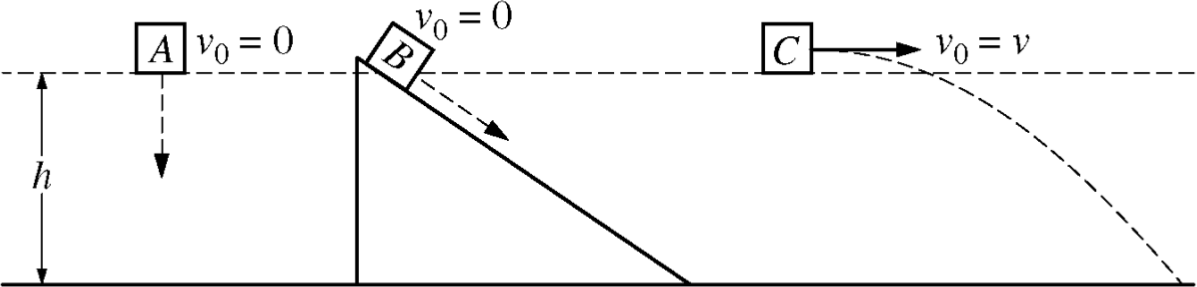
\includegraphics[height=2cm]{blocks.png}
		
Three identical blocks each take a different path from a height h to the ground.  Block A is released from rest and falls vertically.  Block B is released from rest and slides down a frictionless incline.  Block C is projected horizontally with an initial speed v.  
	

\begin{question}
Which block takes the longest time to reach the ground?
\choice{Block A}
\choice{Block B}
\choice{Block C}
\choice{All three blocks reach the ground at the same time.}

	\end{question}

\begin{question}
Which block has the greatest speed just before it hits the ground?
\choice{Block A}
\choice{Block B}
\choice{Block C}
\choice{All three blocks have the same speed just before they hit the ground.}
	\end{question}



\end{block}

\begin{question}
The figure below shows the path of a stunt-car as it drives off a cliff.  Compared to the horizontal component of the car's velocity at point A, the horizontal component of the car's velocity at point B is - 

	\hspace{3in} 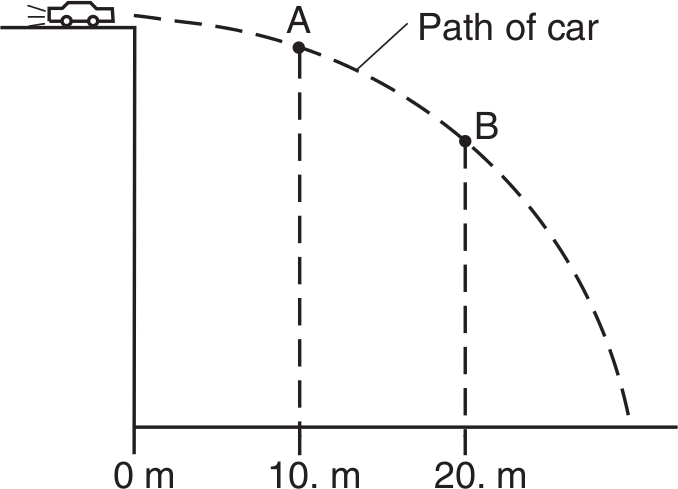
\includegraphics[height=2.5cm]{car.png}
\vspace{-.7in}
\choice{Greater}
\choice{Smaller}
\choice{The Same}
\choice{it cannot be determined without knowing the car's initial velocity.}
\choice{It cannot be determined without knowing the car's vertical velocity at either A or B.}
\end{question}



\end{multiplechoice}

\begin{multiplechoice} [title={Multiple Correct Multiple Choice},
	rearrange=no]
	\textit{For the following question, \textbf{choose two} correct answers.  No credit will be given for incorrect or partially correct answers.  Mark \textbf{both} answers clearly.} 



\begin{question}
	When a projectile is launched horizontally, which of the following statements are true?
	\choice {The vertical acceleration is equal to 9.81 m/s\textsuperscript{2}}
	\choice {The initial horizontal velocity is zero.}
	\choice {The initial vertical velocity is zero.}
	\choice {The horizontal final velocity is equal to the vertical acceleration.}
\end{question}







\end{multiplechoice}

\begin{shortanswer}[title={Free Response}]
\begin{question}
	An accident investigator finds that a car has driven off the edge of Scenic Drive and off of a cliff.  The investigator is given the task of determining whether the car was driving faster than the speed limit, which was 20 mph (8.9408 m/s) in that area.  He may make any measurements that he needs.  
	\begin{enumerate}
		\item In a clear, concise paragraph describe the process that the investigator should use to determine the initial speed of the car, and any measurements he should make.  
		\vspace{2in}
		\item{The investigator measures that the cliff is 52 meters high, and the car landed 37 meters from the cliff.  Complete the following table:}
		
		\begin{center}
			\begin{tabular} {| c | c | }
				\hline
				$x$ = \hspace{0.4in}    & $y $= \hspace{0.4in} \\
				\hline
				$v_{ix}$  = \hspace{0.4in}  &$v_{iy}$  = \hspace{0.4in} \\
				\hline
				$v_{fx}$  = \hspace{0.4in}  &$v_{fy}$  = \hspace{0.4in} \\
				\hline
				$a_{x}$  = \hspace{0.4in}  &$a_{y}$  = \hspace{0.4in} \\
				\hline 
				\multicolumn{2}{|c|}{	$t$  = \hspace{0.4in} }  \\
				\hline
			\end{tabular} 
		\end{center}
	\item{Determine the angle of impact of the car.}
	\vspace{1in}
	\item{Was the car speeding?}
		
	\end{enumerate}
	\end{question}

	\end{shortanswer}

\end{document}



